\newcommand{\theory}{

\part{Theory}

\section{Brief Introduction to Semiconductors}

In the world of material science, semiconductors have occupied researchers for centuries and the fascination continues to this day. According to \citet{Busch1989} the word \textit{semiconductor} was first mentioned by Alessandro Volta in 1782 \textit{"...in a paper read in English before the Royal Society in London on 14 March 1782"}.\citep{Busch1989} Later, Michael Faraday would prove the semiconducting properties of materials by showing that increasing temperature could drastically increase the conductivity in certain materials; why this is i will elaborate further on at a later stage.

The photovoltaic (PV) effect, and subsequently photoelectrocemistry, was discovered only a few decades later in 1839 by Edmond Becquerel when he was able to detect a voltage between a solid material and a liquid electrolyte under illumination. \citep{Becquerel1839}

	\begin{quotation}
		\textit{Dans le dernier Mémoire que j'ai eu l'honneur de présenter à l'Academie, dans sa séance de lundi 29 juliet 1839, je me suis attaché à mettre en évidence, à l'aide des courants électriques, les réactions chimiques qui ont lieu au contact de deux liquides, sous l'influence de la lumière solaire. }
		\end{quotation}\vspace*{-.5cm}
		\begin{flushright}
		\textit{- E. Becquerel, 1839}
	\end{flushright}

%With that the foundation for the photovoltaic effect, and subsequently photoelectrocemistry, was laid. What Becquerel showed was that with two Pt

%Already in 1839, A. E. Becquerel reported observation of a voltage between a solid and a liquid electrolyte when struck by light, the photovoltaic effect

%Another important milestone in the history of semiconductors comes with Ferdinand Braun in 1874 when he, at the age of 24, discover the rectification effect at the point of contact between metals and certain crystal materials. This discovery would not find its practical use until the early 1900's when it became an essential part in the development of the radio. This discovery earned Braun the Nobel Prize in physics in 1909. 


\section{Understanding the Semiconductor}

The basic idea of semiconductors is easiest explained by showing how atoms and the corresponding electron energies behave when bonding to other atoms, going from single atom electron energies through more complex \textit{energy levels} in molecules to \textit{energy bands} in solids. Electrons are only allowed to occupy certain energies, or states, and whether these states are filled or not depends on the energy of the electron in question. The number of electrons allowed at given energies, or rather the density of allowed energies, \intextnote{insert DOS.plot} are called \textit{density of states}; DOS for short.

	\begin{figure}[ht!]
		\centering
		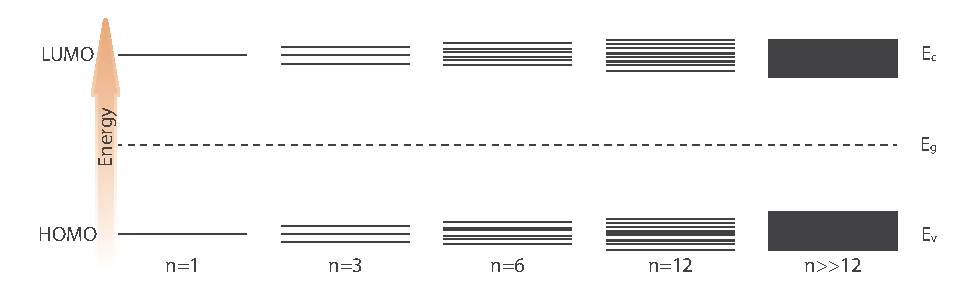
\includegraphics[scale=1]{Figures/Energy_bands1.eps}
		\caption{Schematics showing energy bands for different number of atoms}
		\label{fig:energy_bands}
	\end{figure}

Figure \ref{fig:energy_bands} depicts these allowed energies, each line corresponding to an allowed energy, and shows how they overlap to form bands when a high number of atoms come together to form a bulk material. This is a very simplified model where electrons are treated as free electrons. This is never the case in solids however and to 

%Taking this one step further a reciprocal energy space is added to the system and 

The semiconductor differs from metals in that energy bands are separated in the area around an important energy level called Fermi level, $E_f$, typically by \intextnote{insert number plus ref.} forming a gap in the allowed energies called the \textit{bang gap}, $E_g$; this discontinuity is also observed in the DOS plot shown in fig \intextnote{ref DOS.plt}. 

%%%%%%%% FERMI LEVEL %%%%%%%%%%%%%%%%

To further discuss this concept let me properly introduce this new parameter, $E_f$. Since electrons in solids obey \textit{Fermi-Dirac} statistics\footnote{Fermi-Dirac statistics builds on quantum mechanical principles such as indistinguishably of electrons and the wave nature of electrons. Further details on Fermi-Dirac statistics will not be given in this text. Readers are directed to more comprehensive texts on the subject, such as \citet{Schroeder1999} and \citet{Kittel2004}}  it is possible to show that the distribution of electrons over a range of allowed energies $E$ at thermal equilibrium is

	\begin{align}
		f(E) \eq \dfrac{1}{1+\exp{(E-E_f)/kT}}
		\label{eq:fermi-dirac-distribution}
	\end{align}

where $k$ is Boltzmann's constant\footnote{$k\eq 8.62\e{-5}\ben{eVK}^{-1}$}. Equation \ref{eq:fermi-dirac-distribution} gives the probability that an available state is filled or not at absolute temperature $T$. When $E\eq E_f$

	\begin{align*}
		f(E) \eq \dfrac{1}{1+\exp{(E_f-E_f)/kT}} \eq \dfrac{1}{1+1} \eq \dfrac{1}{2}
	\end{align*}

one of the 'definitions' of the Fermi level materialize: the probability of having an electron occupy the energy state corresponding to the Fermi level is 50\%. \citep{Streetman2015} Another simplified way to explain Fermi energy level is that the Fermi level equals the potential of electrons in the solid at 0 K.

%%%%%%%% figure: Fermi_DOS %%%%%%%%%%%%%%%%

	\begin{wrapfigure}{l}{0.35\textwidth}
		\centering
		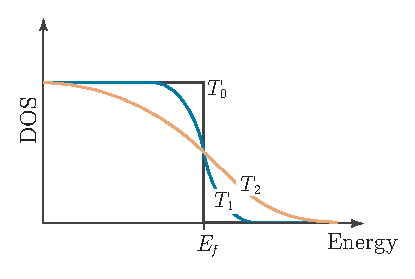
\includegraphics[scale=1]{Figures/Fermi_DOS.eps}
		\caption{$T_0 =0\ben{K}$}
		\label{fig:fermi_DOS}
	\end{wrapfigure}

At 0 K all electrons are therefore confined to what is called the \textit{valence band}, $E_v$, because, in semiconductors, the Fermi level is located in the band gap per definition. The first unoccupied band above the Fermi level is called the conduction band $E_c$, and is consequently empty at 0 K. The Fermi level does get more interesting however when the temperature is not zero. As shown in figure \ref{fig:fermi_DOS}, as temperature increase electrons gain energy and the jump, or \textit{excitation},  to higher empty energy states are possible. In practice this means that electrons are able to make the jump from the valence band to the conduction band as long as the energy provided is sufficient and it is this effect Michael Faraday discovered.

In intrinsic semiconductors the Fermi level resides in the middle of the band gap. However most materials, including semiconductors, are in practice extrinsic, meaning that the material is doped. This results in shifting the Fermi level either towards the valence band in p-type semiconductors or the conduction band in n-type semiconductors. This shift leads to a 

One important point to make at his point is that other types of energy provided to the system has the same effect on electrons, such as in photovoltaics where electrons are excited by the incident photon energy often corresponding to $E_g$, ultimately providing a current in an appropriate circuit. The same can be said about photocatalysis where electrons are excited in the same way, but the electrons are not used to induce a current but rather use the gained electron- or hole energy to catalyze reactions.



\begin{figure}[ht!]
\centering
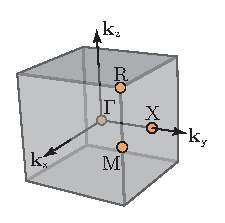
\includegraphics[scale=1]{Figures/1stBZ_cu2o.eps}
\end{figure}

%%%%%%%% figure: Parabolic Energy %%%%%%%%%%%%%%%%



\newpage
\section{Electrochemistry}{
The current in liquid electrolytes are carried by ions created by dissociation of salts in polar solvents. 

\subsection{Pourbaix Diagrams}

Pourbaix diagrams project multiple electrode and electrolyte conditions onto a two dimensional plane and provides information on the corroding conditions as first described by Marcel Pourbaix in his theses dated 1945 \citep{Pourbaix1945}. The two dimensional plot generally depicts three different areas of thermodynamic stability: immunity, passivity and corrosion  as shown in figure \ref{fig:pourbaix_generic}.

%%%%%%%% figure: Pourbaix_generic %%%%%%%%%%%%%%%%
	\begin{wrapfigure}{l}{0.5\textwidth}
		\centering
		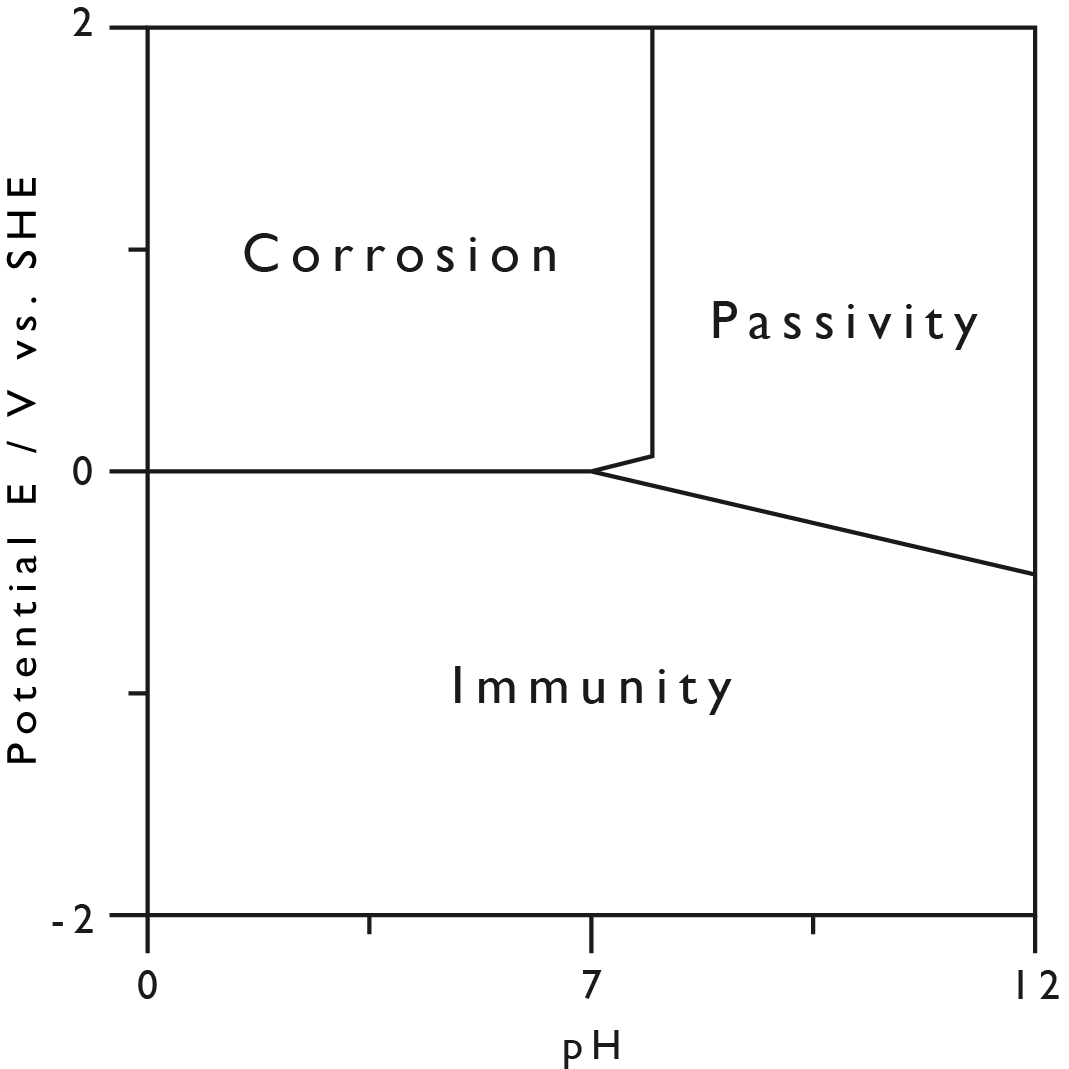
\includegraphics[scale=1]{Figures/pourbaix_generic}
		\caption{Generic Pourbaix diagram for copper}
		\label{fig:pourbaix_generic}
	\end{wrapfigure}
%%%%%%%% end_figure: Pourbaix_generic %%%%%%%%%%%%

The \textit{immunity} zone describes the conditions where the metal itself is the stable phase and corrosion is non-existent. \textit{Passivity} describes the conditions under which the metal is passivated by formation of a coating, usually an oxide or hydroxide. In the corrosion zone, the thermodynamically stable species is a dissolved reaction product, namely metal cations suspended in the aqueous electrolyte \citep{Beverskog1995}.

In a two electrode set-up, one electrode would 


}
\newpage
\section{Quantum mechanical modeling}

Modeling of complex structures and systems has become more readily accessible with time as the computational power of the world has increased at an incredible rate. Also a lot of effort has been made to optimize these calculations and materials scientist today are preforming calculations on large systems with complex structural interactions with high accuracy. The results of these calculations are sometimes impossible to obtain from experimental data and often provide invaluable information. 

This section is to a large extent adopted from the comprehensive book on density functional theory by \citet{Sholl2009}

\subsection{Many Particle Schrödinger Equation}

One of the fundamental things we want to solve is the energy of atoms and \textit{the change in energy} as we move them around. The many particle Schrödinger equation (SE) can, in theory, be used to describe such system with interacting atoms. The simplest form of the time independent, nonrelativistic SE is

\begin{align}
\hat{H}\psi\eq E\psi
	\label{eq:schrödinger_simple}
\end{align}

where $\hat{H}$ is the Hamiltonian operator and $\psi$ is a set of eigenstates of the Hamiltonian, all with an associated eigenvalue $E$; a real number satisfying the eigenvalue equation.

The situation of interest to us, a many-particle system, we need to apply a Hamiltonian to tackle all these interactions.

\begin{align}
\hat{H}\eq \dfrac{h^2}{2m}\sum_{i=1}^{N}\nabla^2_i\,+\, \sum_{i=1}^{N}V(\vec{r}_i) \,+\, \sum_{i=1}^{N}\sum_{j<1}U(\vec{r}_i,\vec{r}_i)
	\label{eq:Hamiltonian}
\end{align}

$m$ being the electron mass, $h$ Planck's constant\footnote{$h\eq6.62\e{-34}\ben{Js}$} and $N$ the number of atoms in the system. The sums represent the kinetic energy of electrons, interaction energy between electron $i$ and the nuclei, and the electron-electron interaction, respectively. The energy $E$ in equation \ref{eq:schrödinger_simple} is the ground state energy of the electrons.

Electron wave functions in systems like these interact, but to such small extent that approximating the total wave function $\psi$ to a product of individual electron wave functions are possible

\begin{align}
\psi\eq \psi_1(\vec{r})\psi_2(\vec{r})\psi_3(\vec{r}) \,...\, \psi_N(\vec{r})
\end{align}

Expressing the wave function like this is know as a Hatree product, but as shown in equation \ref{eq:Hamiltonian}, the electron-electron interaction is crucial to solving SE so solving SE by using the Hartree product approach means solving every electron wave function with respect to all the others, a job requiring massive computational power.

Further, the density of electrons at any point in space can be expressed by means of the individual electron wave function, $\psi_i(\vec{r})$, through 

\begin{align}
n(\vec{r})\eq 2 \sum_i \psi_i^*(\vec{r})\psi_i(\vec{r})
\label{eq:electron_density}
\end{align}

such that the term inside the summation is the probability that an electron with corresponding wave function $\psi_i(\vec{r})$ is located at $\vec{r}$; the factor of 2 accounting for Paulis exclusion principle, allowing two electrons of different spin to occupy the same wave function. The fact that the electron density $n(\vec{r})$ at any point is a function of only three coordinates will prove extremely useful in calculations of SE 

%As the nucleus and electron mass differs immensely; the nucleus being 1800 times more heavy than the electron, we can split this problem in two parts. First the \textit{ground state }of electrons are solved by finding the lowest energy configuration of these electrons moving in the field of atomic nuclei at fixed positions. The separation of these two problems are called Born-Oppenheimer approximation

%
\subsection{Density Functional Theory}

The field of density functional theory (DFT) is basically founded on two mathematical theorems by Kohn and Hohenberg \citep{Hohenberg1964}, and the Kohn-Sham equation\citep{Kohn1965}. The first theorem states that \textit{the ground-state energy from SE is a unique functional of the electron density}; there is a one-to-one mapping between the wave function of the ground state and electron density in this state. This means that the ground state energy $E$ can be expressed as
\begin{align}
E\fpara{n(\vec{r})}
\end{align}
where $n(\vec{r})$ is the electron density, hence \textbf{density functional theory}. In practice this means that solving SE is possible by finding a function of three variables rather than $3N$ variables, since the ground state electron density uniquely determine all properties, including the energy and wave function. 

The problem with this theroem is that although it states that a functional like this exist, it does not declare what this functional is, although an important property of this functional is defined in the second Hohenberg-Kohn theorem: \textit{The electron density that minimizes the energy of the overall functional is the true electron density corresponding to the full solution of SE}, meaning that if the 'correct' functional were known, varying the electron density and subsequently finding an energetic minimum in the system would yield the relevant electron density; this \textit{variation principle} is what is practically implemented in computational functional calculations such as PBE, PBE0, HSE06 etc.

Using that the electron density, $n(\vec{r})$, are defined by the single 
}
